\section{Beállítások menü}

\begin{figure}
\centering
  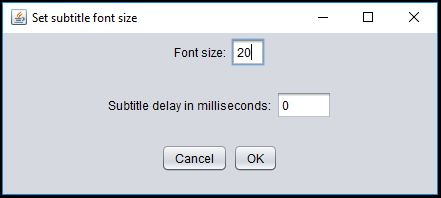
\includegraphics[width=0.8\linewidth]{images/options.jpg}
  \caption{Beállítások ablak}
  \label{fig:options}
\end{figure}

Miután a fő funkciók megvalósításával elkészültem, néhány apró kényelmi kiegészítő funkciót is implementáltam. Név szerint a felirat betűméretének állítását, illetve a felirat késleltetést. Ezek egy \textit{Options} ablakban kaptak helyet, amely \ref{fig:options}-es ábrán látható.

A lejátszó felső menüsávjában megtalálható \textit{Options} menüpontra kattintva jeleníthető meg a beállításokat tartalmazó ablak. Felül, a \textit{Font size} felirat mellett lévő beviteli mezőben a felirat méretét, az alatta lévő \textit{Subtitle delay in milliseconds} mellett található mezőben pedig a felirat késleltetését állíthatjuk milliszekundumos pontossággal. A változtatások elvetése a \textit{Cancel}, mentése az \textit{OK} gomb megnyomásával történik. Mindkét esetben az alkalmazás egy-egy statikus változó értékét írja felül. A \textit{SubtitleOverlay} osztály a feliratok megjelenítése során ezen változók értékeit használja.

\begin{lstlisting}[caption=Feliratok késleltetése, label={lst:delay}, language=java]
public void update(boolean force) {
   //...
   //subtitle delay
   long time = mediaPlayer.getTime() + subtitleDelay;
   //...
}
\end{lstlisting}

Késleltetés módosítása esetén a függvény törzsében (\ref{lst:delay}), amely a feliratok képernyőn történő frissítését végzi, az aktuális időhöz hozzáadjuk a beállított késleltetést. Így a felirat időzítése a kívánt értékkel elcsúszik. Az eltolás mindkét irányban lehetséges, attól függően, hogy pozitív, vagy negatív értékkel rendelkezik a \textit{subtitleDelay}. Csak egész számok adhatóak meg, alapértelmezett értéke nulla.


\begin{lstlisting}[caption=Feliratok mérete, label={lst:fontsize}, language=java]
public void paint(Graphics g) {
	//...
	g2.setFont(new Font("Serif", Font.PLAIN, fontSize));
	//...
}
\end{lstlisting}

Betűméret módosítása esetén a feliratokat kirajzoló metódus törzsében történik a módosítás, hiszen a betűméretet értékét egy statikus változóból olvassa ki az alkalmazás (\ref{lst:fontsize}). A megjelenített szöveg így a megadott méretűre változik. Fontos megemlíteni, hogy csak egész, nullánál nagyobb betűméret adható meg, egyéb esetben az alkalmazás hibaüzenetet jelenít meg. Alapértelmezett értéke 20, amely ablakos megjelenítésnél elegendő lehet, azonban teljes képernyős módban legtöbbször kevés, így ajánlott ennek módosítása. A feliratok méretének állítására gyorsbillentyűk is használhatók. Nagyításra a \textit{Ctrl +}, kicsinyítésre pedig a \textit{Ctrl -} billentyűkombinációk alkalmasak.

A két segédfunkcióval a feliratozás pontossága minden esetben biztosítható, hiszen, ha a feliratfájl esetlegesen téves időpillanatokat, vagy a médiafájl csúszást tartalmaz, akkor ezek orvosolhatóak a bemutatott funkcióval. Emellett pedig a felirat láthatósága is mindig biztosítható a betűméret módosításával.